
The analysis of tensegrity structures is non trivial, so there is a very specialized method of computing the parameters associated with the members of the structure.
We'll begin reviewing the static analysis of a tensegrity in order to get the equilibrium conditions of the structure.

\subsection{Stability analysis of a 2-bar and 6-element tensegrity}


Given the following configuration, we want to know the internal forces
necessary for the system to be in equilibrium.

\begin{figure}[htbp]
    \centering
    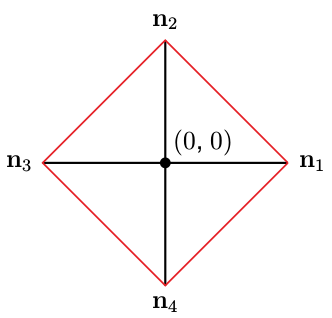
\includegraphics{imagenes/7-tensegril/PlanarTensegrity.png}
\end{figure}

We know that in a static structure the sum of the internal forces must
be equal to \(0\), so the first thing that we have to obtain is a \(F\)
that represents the sum of the internal forces.

We will begin by importing the symbolic calculus library

\begin{Verbatim}[commandchars=\\\{\}]
    {\color{incolor}In [{\color{incolor}1}]:} \PY{k+kn}{from} \PY{n+nn}{sympy} \PY{k+kn}{import} \PY{n}{init\PYZus{}printing}\PY{p}{,} \PY{n}{var}\PY{p}{,} \PY{n}{Matrix}\PY{p}{,} \PY{n}{solve}
\end{Verbatim}

\begin{Verbatim}[commandchars=\\\{\}]
    {\color{incolor}In [{\color{incolor}2}]:} \PY{n}{init\PYZus{}printing}\PY{p}{(}\PY{p}{)}
\end{Verbatim}

And initializing the symbolic variables that represent the internal
forces on the nodes.

\begin{Verbatim}[commandchars=\\\{\}]
    {\color{incolor}In [{\color{incolor}3}]:} \PY{n}{var}\PY{p}{(}\PY{l+s}{\PYZdq{}}\PY{l+s}{lambda:3}\PY{l+s}{\PYZdq{}}\PY{p}{)}
    \PY{n}{var}\PY{p}{(}\PY{l+s}{\PYZdq{}}\PY{l+s}{gamma:5}\PY{l+s}{\PYZdq{}}\PY{p}{)}\PY{p}{;}
\end{Verbatim}

We define the vectors that describe the nodes:

\begin{Verbatim}[commandchars=\\\{\}]
    {\color{incolor}In [{\color{incolor}4}]:} \PY{n}{n1} \PY{o}{=} \PY{n}{Matrix}\PY{p}{(}\PY{p}{[}\PY{l+m+mi}{1}\PY{p}{,} \PY{l+m+mi}{0}\PY{p}{]}\PY{p}{)}
    \PY{n}{n2} \PY{o}{=} \PY{n}{Matrix}\PY{p}{(}\PY{p}{[}\PY{l+m+mi}{0}\PY{p}{,} \PY{l+m+mi}{1}\PY{p}{]}\PY{p}{)}
    \PY{n}{n3} \PY{o}{=} \PY{n}{Matrix}\PY{p}{(}\PY{p}{[}\PY{o}{\PYZhy{}}\PY{l+m+mi}{1}\PY{p}{,} \PY{l+m+mi}{0}\PY{p}{]}\PY{p}{)}
    \PY{n}{n4} \PY{o}{=} \PY{n}{Matrix}\PY{p}{(}\PY{p}{[}\PY{l+m+mi}{0}\PY{p}{,} \PY{o}{\PYZhy{}}\PY{l+m+mi}{1}\PY{p}{]}\PY{p}{)}

    \PY{n}{N} \PY{o}{=} \PY{p}{(}\PY{p}{(}\PY{n}{n1}\PY{o}{.}\PY{n}{row\PYZus{}join}\PY{p}{(}\PY{n}{n2}\PY{p}{)}\PY{p}{)}\PY{o}{.}\PY{n}{row\PYZus{}join}\PY{p}{(}\PY{n}{n3}\PY{p}{)}\PY{p}{)}\PY{o}{.}\PY{n}{row\PYZus{}join}\PY{p}{(}\PY{n}{n4}\PY{p}{)}
    \PY{n}{N}
\end{Verbatim}
\texttt{\color{outcolor}Out[{\color{outcolor}4}]:}


\begin{equation*}
    \left[\begin{matrix}1 & 0 & -1 & 0\\0 & 1 & 0 & -1\end{matrix}\right]
\end{equation*}



So the vectors that describe the bars are:

\begin{Verbatim}[commandchars=\\\{\}]
    {\color{incolor}In [{\color{incolor}5}]:} \PY{n}{b1} \PY{o}{=} \PY{n}{n3} \PY{o}{\PYZhy{}} \PY{n}{n1}
    \PY{n}{b2} \PY{o}{=} \PY{n}{n4} \PY{o}{\PYZhy{}} \PY{n}{n2}

    \PY{n}{B} \PY{o}{=} \PY{n}{b1}\PY{o}{.}\PY{n}{row\PYZus{}join}\PY{p}{(}\PY{n}{b2}\PY{p}{)}
    \PY{n}{B}
\end{Verbatim}
\texttt{\color{outcolor}Out[{\color{outcolor}5}]:}


\begin{equation*}
    \left[\begin{matrix}-2 & 0\\0 & -2\end{matrix}\right]
\end{equation*}



And the strings are characterized by:

\begin{Verbatim}[commandchars=\\\{\}]
    {\color{incolor}In [{\color{incolor}6}]:} \PY{n}{s1} \PY{o}{=} \PY{n}{n2} \PY{o}{\PYZhy{}} \PY{n}{n1}
    \PY{n}{s2} \PY{o}{=} \PY{n}{n3} \PY{o}{\PYZhy{}} \PY{n}{n2}
    \PY{n}{s3} \PY{o}{=} \PY{n}{n4} \PY{o}{\PYZhy{}} \PY{n}{n3}
    \PY{n}{s4} \PY{o}{=} \PY{n}{n1} \PY{o}{\PYZhy{}} \PY{n}{n4}

    \PY{n}{S} \PY{o}{=} \PY{p}{(}\PY{p}{(}\PY{n}{s1}\PY{o}{.}\PY{n}{row\PYZus{}join}\PY{p}{(}\PY{n}{s2}\PY{p}{)}\PY{p}{)}\PY{o}{.}\PY{n}{row\PYZus{}join}\PY{p}{(}\PY{n}{s3}\PY{p}{)}\PY{p}{)}\PY{o}{.}\PY{n}{row\PYZus{}join}\PY{p}{(}\PY{n}{s4}\PY{p}{)}
    \PY{n}{S}
\end{Verbatim}
\texttt{\color{outcolor}Out[{\color{outcolor}6}]:}


\begin{equation*}
    \left[\begin{matrix}-1 & -1 & 1 & 1\\1 & -1 & -1 & 1\end{matrix}\right]
\end{equation*}



Before defining the conectivity matrix, we begin by defining \(n\)
vectors \(e_i\) with dimension \(n\), where \(n\) is the number of nodes
in the structure, and the element \(i\) in the vector is \(1\) while the
rest are all \(0\)'s.

\begin{Verbatim}[commandchars=\\\{\}]
    {\color{incolor}In [{\color{incolor}7}]:} \PY{n}{e1} \PY{o}{=} \PY{n}{Matrix}\PY{p}{(}\PY{p}{[}\PY{l+m+mi}{1}\PY{p}{,} \PY{l+m+mi}{0}\PY{p}{,} \PY{l+m+mi}{0}\PY{p}{,} \PY{l+m+mi}{0}\PY{p}{]}\PY{p}{)}
    \PY{n}{e2} \PY{o}{=} \PY{n}{Matrix}\PY{p}{(}\PY{p}{[}\PY{l+m+mi}{0}\PY{p}{,} \PY{l+m+mi}{1}\PY{p}{,} \PY{l+m+mi}{0}\PY{p}{,} \PY{l+m+mi}{0}\PY{p}{]}\PY{p}{)}
    \PY{n}{e3} \PY{o}{=} \PY{n}{Matrix}\PY{p}{(}\PY{p}{[}\PY{l+m+mi}{0}\PY{p}{,} \PY{l+m+mi}{0}\PY{p}{,} \PY{l+m+mi}{1}\PY{p}{,} \PY{l+m+mi}{0}\PY{p}{]}\PY{p}{)}
    \PY{n}{e4} \PY{o}{=} \PY{n}{Matrix}\PY{p}{(}\PY{p}{[}\PY{l+m+mi}{0}\PY{p}{,} \PY{l+m+mi}{0}\PY{p}{,} \PY{l+m+mi}{0}\PY{p}{,} \PY{l+m+mi}{1}\PY{p}{]}\PY{p}{)}
\end{Verbatim}

So, by making the same operations as before, but with the vectors
\(e_i\), we'll obtain the matrix \(D\) which is the transpose of the
\(C\) matrix.

\begin{Verbatim}[commandchars=\\\{\}]
    {\color{incolor}In [{\color{incolor}8}]:} \PY{n}{d1} \PY{o}{=} \PY{n}{e3} \PY{o}{\PYZhy{}} \PY{n}{e1}
    \PY{n}{d2} \PY{o}{=} \PY{n}{e4} \PY{o}{\PYZhy{}} \PY{n}{e2}
    \PY{n}{d3} \PY{o}{=} \PY{n}{e2} \PY{o}{\PYZhy{}} \PY{n}{e1}
    \PY{n}{d4} \PY{o}{=} \PY{n}{e3} \PY{o}{\PYZhy{}} \PY{n}{e2}
    \PY{n}{d5} \PY{o}{=} \PY{n}{e4} \PY{o}{\PYZhy{}} \PY{n}{e3}
    \PY{n}{d6} \PY{o}{=} \PY{n}{e1} \PY{o}{\PYZhy{}} \PY{n}{e4}

    \PY{n}{D} \PY{o}{=} \PY{p}{(}\PY{p}{(}\PY{p}{(}\PY{n}{d1}\PY{o}{.}\PY{n}{row\PYZus{}join}\PY{p}{(}\PY{n}{d2}\PY{p}{)}\PY{p}{)}\PY{o}{.}\PY{n}{row\PYZus{}join}\PY{p}{(}\PY{n}{d3}\PY{p}{)}\PY{p}{)}\PY{o}{.}\PY{n}{row\PYZus{}join}\PY{p}{(}\PY{n}{d4}\PY{p}{)}\PY{p}{)}\PY{o}{.}\PY{n}{row\PYZus{}join}\PY{p}{(}\PY{n}{d5}\PY{p}{)}\PY{o}{.}\PY{n}{row\PYZus{}join}\PY{p}{(}\PY{n}{d6}\PY{p}{)}

    \PY{n}{C} \PY{o}{=} \PY{n}{D}\PY{o}{.}\PY{n}{T}
    \PY{n}{C}
\end{Verbatim}
\texttt{\color{outcolor}Out[{\color{outcolor}8}]:}


\begin{equation*}
    \left[\begin{matrix}-1 & 0 & 1 & 0\\0 & -1 & 0 & 1\\-1 & 1 & 0 & 0\\0 & -1 & 1 & 0\\0 & 0 & -1 & 1\\1 & 0 & 0 & -1\end{matrix}\right]
\end{equation*}



We'll define now a \(\Lambda\) diagonal matrix, being it's elements, the
internal compression forces of the structure.

\begin{Verbatim}[commandchars=\\\{\}]
    {\color{incolor}In [{\color{incolor}9}]:} \PY{n}{Lambda} \PY{o}{=} \PY{n}{Matrix}\PY{p}{(}\PY{p}{[}\PY{p}{[}\PY{n}{lambda1}\PY{p}{,} \PY{l+m+mi}{0}\PY{p}{]}\PY{p}{,} \PY{p}{[}\PY{l+m+mi}{0}\PY{p}{,} \PY{n}{lambda2}\PY{p}{]}\PY{p}{]}\PY{p}{)}
    \PY{n}{Lambda}
\end{Verbatim}
\texttt{\color{outcolor}Out[{\color{outcolor}9}]:}


\begin{equation*}
    \left[\begin{matrix}\lambda_{1} & 0\\0 & \lambda_{2}\end{matrix}\right]
\end{equation*}



\begin{Verbatim}[commandchars=\\\{\}]
    {\color{incolor}In [{\color{incolor}10}]:} \PY{o}{\PYZhy{}}\PY{n}{B}\PY{o}{*}\PY{n}{Lambda}
\end{Verbatim}
\texttt{\color{outcolor}Out[{\color{outcolor}10}]:}


\begin{equation*}
    \left[\begin{matrix}2 \lambda_{1} & 0\\0 & 2 \lambda_{2}\end{matrix}\right]
\end{equation*}



And the \(\Gamma\) diagonal matrix, with it's elements the internal
stress forces.

\begin{Verbatim}[commandchars=\\\{\}]
    {\color{incolor}In [{\color{incolor}11}]:} \PY{n}{Gamma} \PY{o}{=} \PY{n}{Matrix}\PY{p}{(}\PY{p}{[}\PY{p}{[}\PY{n}{gamma1}\PY{p}{,} \PY{l+m+mi}{0}\PY{p}{,} \PY{l+m+mi}{0}\PY{p}{,} \PY{l+m+mi}{0}\PY{p}{]}\PY{p}{,} \PY{p}{[}\PY{l+m+mi}{0}\PY{p}{,} \PY{n}{gamma2}\PY{p}{,} \PY{l+m+mi}{0}\PY{p}{,} \PY{l+m+mi}{0}\PY{p}{]}\PY{p}{,} \PY{p}{[}\PY{l+m+mi}{0}\PY{p}{,} \PY{l+m+mi}{0}\PY{p}{,} \PY{n}{gamma3}\PY{p}{,} \PY{l+m+mi}{0}\PY{p}{]}\PY{p}{,} \PY{p}{[}\PY{l+m+mi}{0}\PY{p}{,} \PY{l+m+mi}{0}\PY{p}{,} \PY{l+m+mi}{0}\PY{p}{,} \PY{n}{gamma4}\PY{p}{]}\PY{p}{]}\PY{p}{)}
    \PY{n}{Gamma}
\end{Verbatim}
\texttt{\color{outcolor}Out[{\color{outcolor}11}]:}


\begin{equation*}
    \left[\begin{matrix}\gamma_{1} & 0 & 0 & 0\\0 & \gamma_{2} & 0 & 0\\0 & 0 & \gamma_{3} & 0\\0 & 0 & 0 & \gamma_{4}\end{matrix}\right]
\end{equation*}



\begin{Verbatim}[commandchars=\\\{\}]
    {\color{incolor}In [{\color{incolor}12}]:} \PY{n}{S}\PY{o}{*}\PY{n}{Gamma}
\end{Verbatim}
\texttt{\color{outcolor}Out[{\color{outcolor}12}]:}


\begin{equation*}
    \left[\begin{matrix}- \gamma_{1} & - \gamma_{2} & \gamma_{3} & \gamma_{4}\\\gamma_{1} & - \gamma_{2} & - \gamma_{3} & \gamma_{4}\end{matrix}\right]
\end{equation*}



It's worth noting that the \(M\) matrix that contains all of the
elements of the structure, can be obtained in two ways.

\[
M = \begin{bmatrix} B & S \end{bmatrix}
\]

\[
M = N C^T
\]

\begin{Verbatim}[commandchars=\\\{\}]
    {\color{incolor}In [{\color{incolor}13}]:} \PY{n}{M} \PY{o}{=} \PY{n}{B}\PY{o}{.}\PY{n}{row\PYZus{}join}\PY{p}{(}\PY{n}{S}\PY{p}{)}
    \PY{n}{M}
\end{Verbatim}
\texttt{\color{outcolor}Out[{\color{outcolor}13}]:}


\begin{equation*}
    \left[\begin{matrix}-2 & 0 & -1 & -1 & 1 & 1\\0 & -2 & 1 & -1 & -1 & 1\end{matrix}\right]
\end{equation*}



\begin{Verbatim}[commandchars=\\\{\}]
    {\color{incolor}In [{\color{incolor}14}]:} \PY{n}{N}\PY{o}{*}\PY{n}{C}\PY{o}{.}\PY{n}{T}
\end{Verbatim}
\texttt{\color{outcolor}Out[{\color{outcolor}14}]:}


\begin{equation*}
    \left[\begin{matrix}-2 & 0 & -1 & -1 & 1 & 1\\0 & -2 & 1 & -1 & -1 & 1\end{matrix}\right]
\end{equation*}



And due to the partition of the matrix
\(M = \begin{bmatrix} B & S \end{bmatrix}\), it simplifies the math of
the matrix \(F\):

\[
F =
\begin{bmatrix}
    -B \Lambda & S \Gamma
    \end{bmatrix} C
    \]

    \begin{Verbatim}[commandchars=\\\{\}]
        {\color{incolor}In [{\color{incolor}15}]:} \PY{n}{F} \PY{o}{=} \PY{p}{(}\PY{o}{\PYZhy{}}\PY{n}{B}\PY{o}{*}\PY{n}{Lambda}\PY{p}{)}\PY{o}{.}\PY{n}{row\PYZus{}join}\PY{p}{(}\PY{n}{S}\PY{o}{*}\PY{n}{Gamma}\PY{p}{)}\PY{o}{*}\PY{n}{C}
        \PY{n}{F}
    \end{Verbatim}
    \texttt{\color{outcolor}Out[{\color{outcolor}15}]:}


    \begin{equation*}
        \left[\begin{matrix}\gamma_{1} + \gamma_{4} - 2 \lambda_{1} & - \gamma_{1} + \gamma_{2} & - \gamma_{2} - \gamma_{3} + 2 \lambda_{1} & \gamma_{3} - \gamma_{4}\\- \gamma_{1} + \gamma_{4} & \gamma_{1} + \gamma_{2} - 2 \lambda_{2} & - \gamma_{2} + \gamma_{3} & - \gamma_{3} - \gamma_{4} + 2 \lambda_{2}\end{matrix}\right]
    \end{equation*}



    So now the only thing left to assume is the fact that the sum of the
    internal forces in each node is \(0\). The next line of code, assumes
    that every entry of the matrix is equal to \(0\), so we only have to put
    tha matrix for it to yield:

    \begin{Verbatim}[commandchars=\\\{\}]
        {\color{incolor}In [{\color{incolor}16}]:} \PY{n}{solve}\PY{p}{(}\PY{n}{F}\PY{p}{)}
    \end{Verbatim}
    \texttt{\color{outcolor}Out[{\color{outcolor}16}]:}


    \begin{equation*}
        \begin{bmatrix}\begin{Bmatrix}\gamma_{1} : \lambda_{2}, & \gamma_{2} : \lambda_{2}, & \gamma_{3} : \lambda_{2}, & \gamma_{4} : \lambda_{2}, & \lambda_{1} : \lambda_{2}\end{Bmatrix}\end{bmatrix}
        \end{equation*}



        Every force must be the same.


\subsection{String Forces}
    %\input{FuerzasdeCuerda.tex}

    Forces on the rod are due to the elongation of strings and ground reactions.
    For simplicity, we assume that the strings are Hookean, and that they are firmly attached to nodes on the rods or on fixed space coordinates.
    That is, strings are linear force elements with rest length $l_i^0$ and stiffness $k_i$.
    The force vector of the $i^{th}$ string is:

    \begin{equation}
        f(n) =
        \begin{cases}
            \hfill 0    \hfill & ||s_i|| < l_1^0 \\
            \hfill \kappa_i \left( ||s_i|| - l_1^0 \right) \left( \frac{s_i}{||s_i||} \right) \hfill & ||s_i|| \ge l_1^0 \\
        \end{cases}
    \end{equation}

    where $s_i$ is a vector in the direction of the $i^{th}$ string.
    String vectors are linear functions of the nodes of the structure as we made it the last section, assembling a matrix of string vectors and nodes.

    \begin{equation}
        S = N C_S^T \quad
        S =
        \begin{pmatrix}
            s_1 & \dots & s_m
        \end{pmatrix} \in \mathbbm{R}^{3 \times m} \quad
        N =
        \begin{pmatrix}
            n_1 & \dots & n_n
        \end{pmatrix} \in \mathbbm{R}^{3 \times n}
        \end{equation}

    where the vector $n_k$ denotes the $k^{th}$ node in the structure and the string connectivity matrix $C_S \in \mathbbm{R}^{m \times n}$, it follows that:

    \begin{equation}
        T = - S \Gamma
    \end{equation}

    where we made use of the diagonal matrix $\Gamma$ which contains the force densities on its diagonal.

    \begin{equation}
        F =
        \begin{pmatrix}
            f_1 & \dots & f_n
        \end{pmatrix} = T C_S = - N C_S^T \Gamma C_S
    \end{equation}

    It follows then, that the matrix F is the matrix of nodal forces.

\subsection{Tensegrity Structures Mechanics}
    %\input{MechanicsofTensegrityStructures.tex}

\subsection{Dynamical Analysis of Tensegrity Structures}

    The dynamics of a tensegrity structure is caracterized by the following equation

    \begin{equation}
        \left( \ddot{Q} + Q \boxminus \right) M = F_Q
    \end{equation}

    where

    \begin{equation}
        Q =
        \begin{pmatrix}
            R & B
        \end{pmatrix} =
        \begin{pmatrix}
            r_1 & \dots & r_k & b_1 & \dots & b_k
        \end{pmatrix}
    \end{equation}

    \begin{equation}
        \boxminus = \text{diag}
        \begin{pmatrix}
            0 & \dots & \xi_1 & \dots & \xi_k
        \end{pmatrix}
    \end{equation}

    \begin{equation}
        M = \text{diag}
        \begin{pmatrix}
            m_1 & \dots & m_k & J_1 & \dots & J_k
        \end{pmatrix}
    \end{equation}

    for $k$ nodes, and $F_Q$ is computed with:

    \begin{equation}
        F_Q = \left( W - Q \Psi^T C_S^T \Gamma C_S \right) \Psi^T
    \end{equation}

    where $W$ is a vector with the external forces applied in each node, $C_S$ is the conectivity matrix for the strings and $\Gamma$ is a matrix with the forces densities in the strings

    So, we can see that the prerequisites to compute the equations of motion for the system are $Q$, $\Psi$, $C_S$ and $\Gamma$.
    In this expressions we can see that $\Psi$, $C_S$ and $\Gamma$ are constant parameters of the system and $Q$, which depends on the geometry of the structure, is the only variable in the equations of motion as they satnd.

    It can be shown that this expression reduces to the following

    \begin{eqnarray}
        m_i \ddot{r}_i & = & f_{r_i} \nonumber \\
        J_i \ddot{b}_i & = & P(b) f_{b_i} - J_i b_i
    \end{eqnarray}

    where $P(b) = I - b_i b_i^T$ is the projection matrix for the orientation vector $b_i$.
